\newcommand{\TODO}[1]{\textbf{[TODO: #1]}}
\chapter{Results: Effective heating rates, relevant nuclei and bolometric luminosities}\label{Results}

This chapter presents the radioactive heating of the 512 trajectories for the three rate sets of Table~\ref{tab:rate_sets} with the identification of the relevant nuclei and the corresponding bolometric luminosity.
The effective heating rates $\dot\varepsilon_x(t)$ of the channels $x\in\{\beta^-,\alpha,\mathrm{fis}\}$ include the thermalization efficiencies of Sec.~\ref{sec:partition}, evaluated for all trajectories with an ejecta mass $M_{\rm ej}=0.05\,M_\odot$ and a velocity corresponding to the trajectory.

The Tian and Zhou sets share the $\alpha$-decay rates and differ only in the $\beta^-$ rates, whereas the ReacLib set differs from both in the two (Sec.~\ref{sec:methods_rates}).
We therefore attribute to the $\beta^-$ rates the differences between Tian and Zhou, and to the decay-rate prescription as a whole the differences between ReacLib and the other two sets.

%------------------------------------------------------------------------------------------
\section{Heating regimes across the parameter space}\label{sec:res_classes}
%------------------------------------------------------------------------------------------

The first result we will show here is Fig.~\ref{fig:heating}.
That figure present the average and the distribution of the effective heating rate for each prescription.
The results clearly suggest that there is no much difference between prescriptions, which is true if we look the whole ensemble.
However, such big spreads, as we will show, hide interesting results.
Since the effective heating is the sum of the contribution from $\alpha$, $\beta^{-}$ decay and fission\footnote{The effective heating rate from fission is taken directly from the main output of WinNet.} we can find the ratios for each channel.
Figure.~\ref{fig:heating_chanels} show such distinction between decay modes and from that we can see that the spread is quite large for the ratios.
\begin{figure}[h]
  \centering
  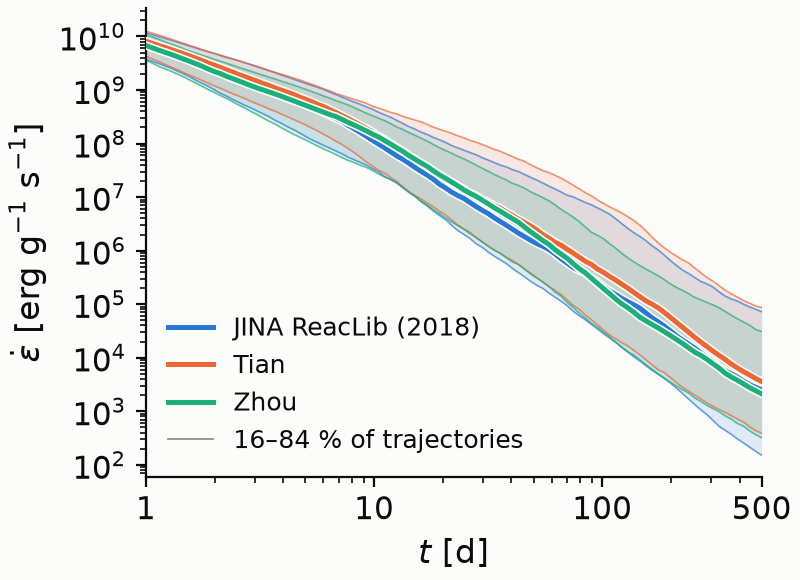
\includegraphics[width=0.7\textwidth]{Figures/heating_bands_sets_therm.png}
  \caption{Average and spread of the total effective heating rate across the whole 512 ensemble per prescription.}
  \label{fig:heating}
\end{figure}
That suggest that some trajectories favors some decay channels.
We saw that behavior in Chapter.~\ref{ch:methods} when we saw the $Y_e$ as a function of time for some trajectories.
Low electron fraction with very high velocities favor the free neutrons instead of heavy nuclei and therefore the $\beta^{-}$ of such neutrons. 
We therefore grouped the trajectories by the similarity\footnote{The classification uses ward hierarchical clustering.} of the time dependence of their ratios $\dot\varepsilon_x/\dot\varepsilon_{total}$, which gives the five classes of Table~\ref{tab:res_classes}.
Figure~\ref{fig:res_class_map} shows where they lie in the parameter space.


\begin{figure}[H]
  \centering
  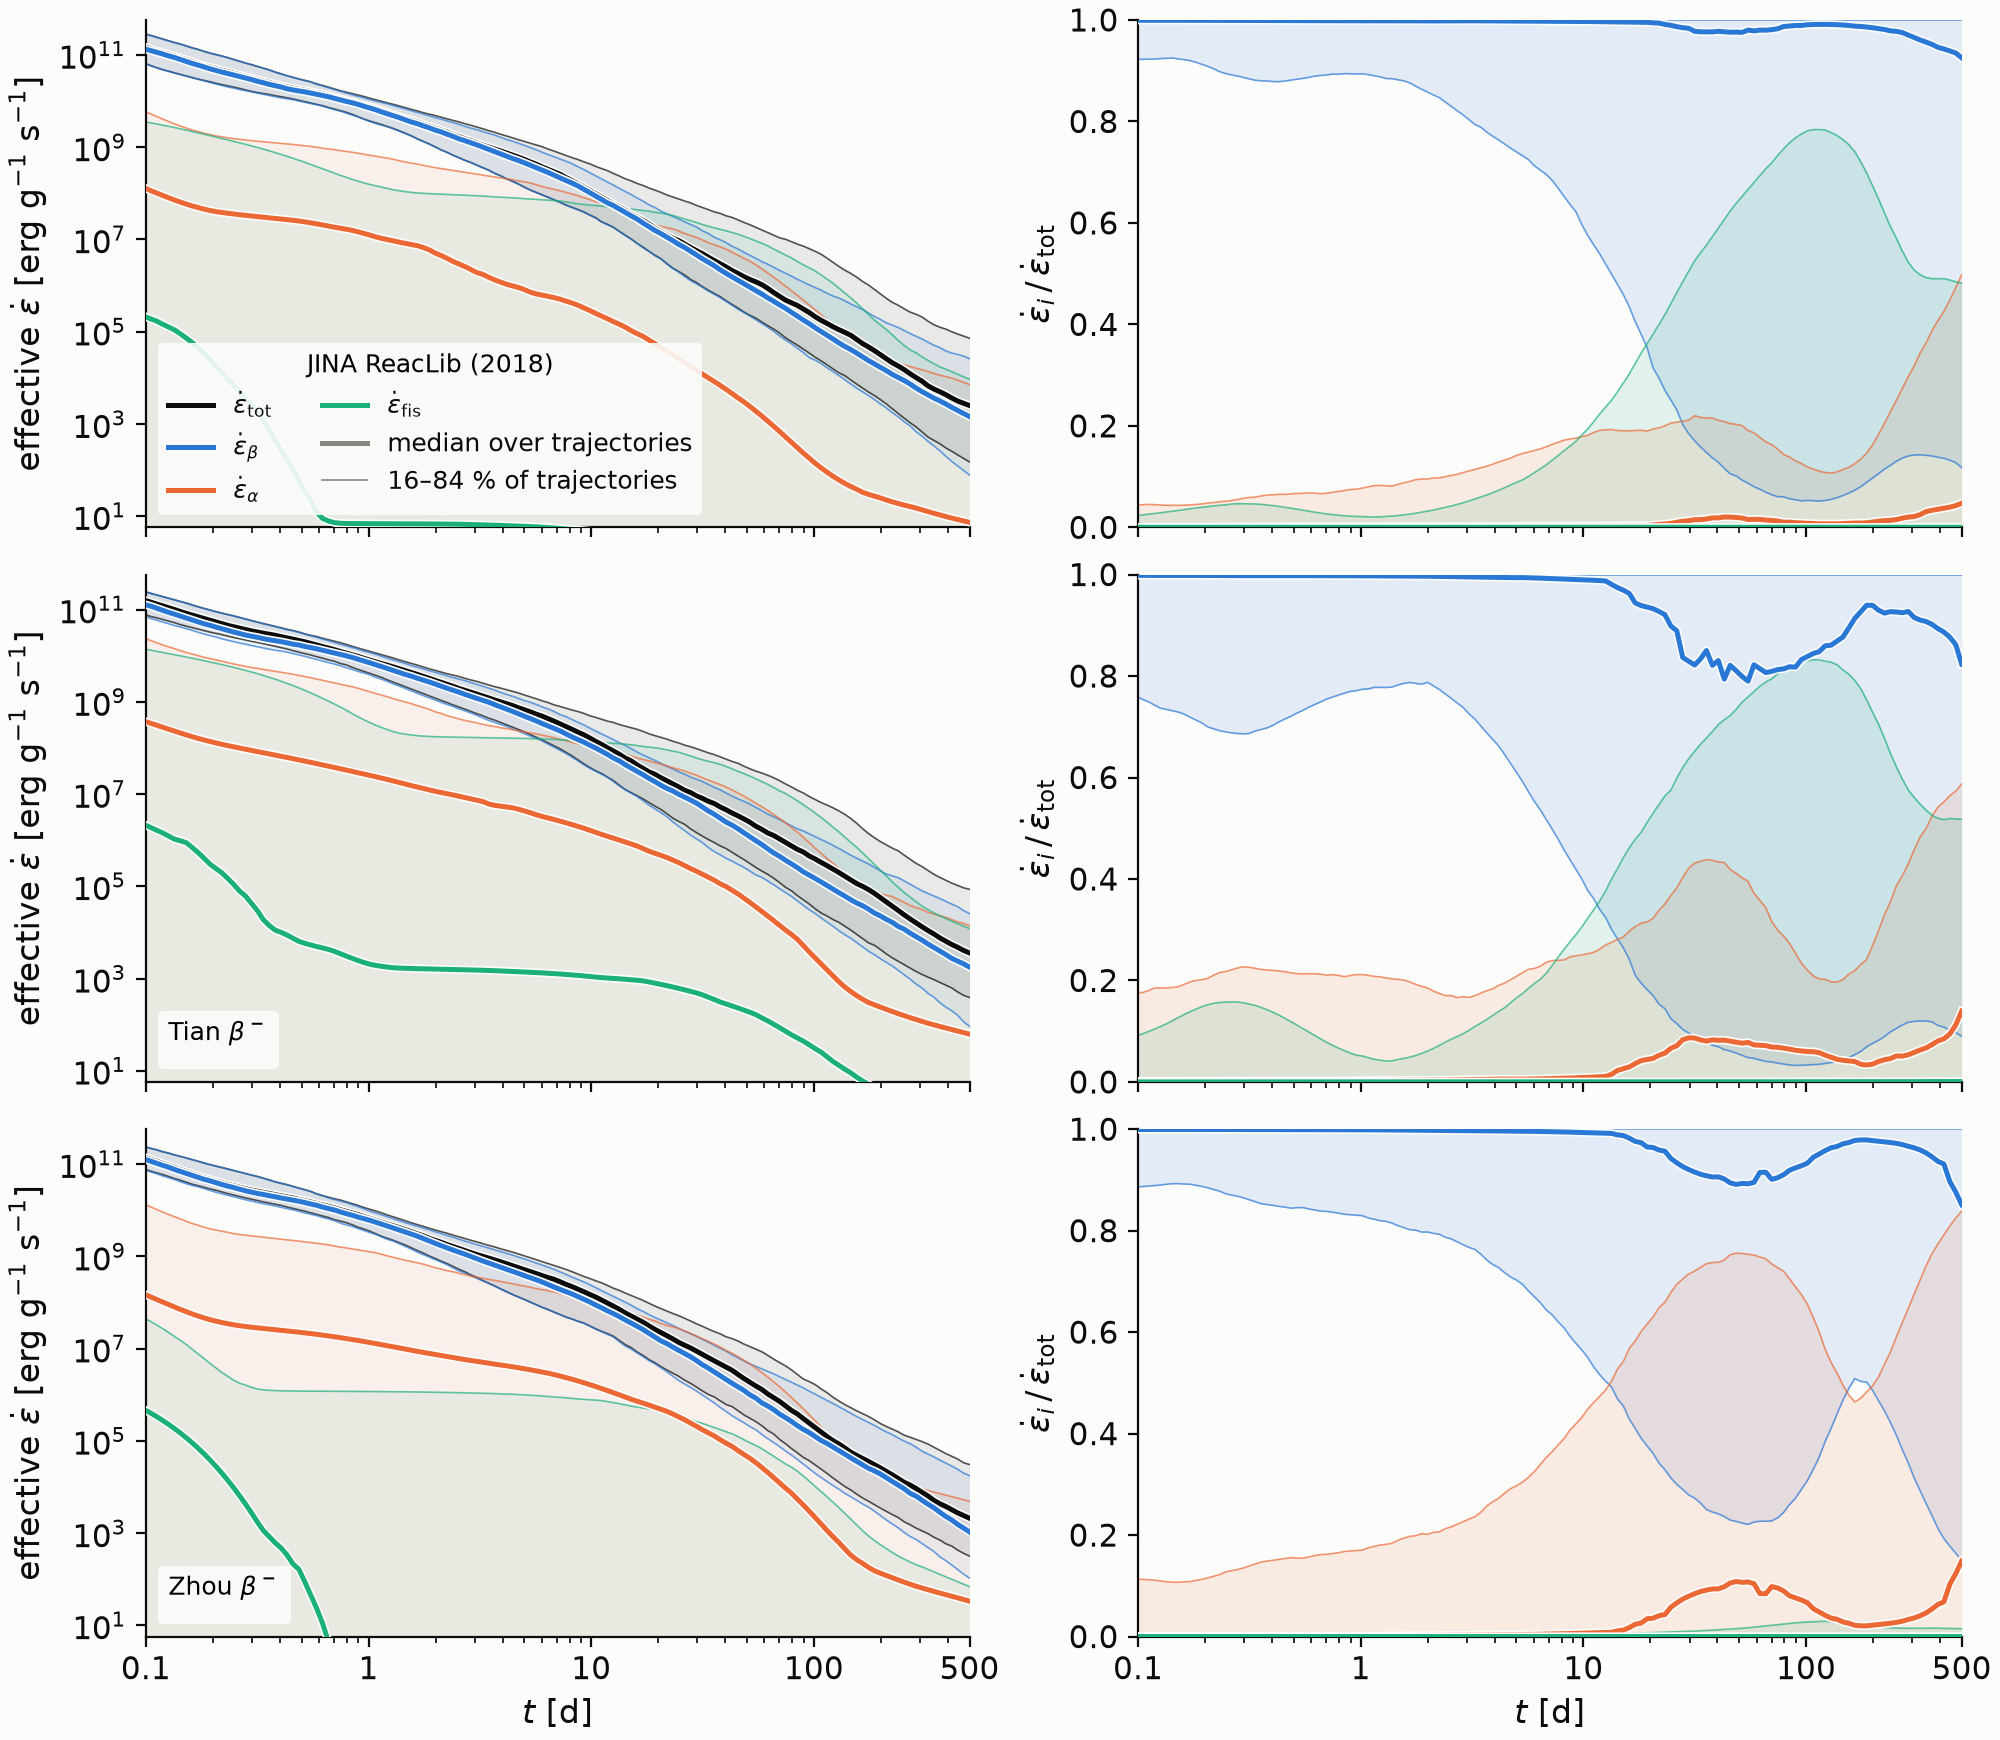
\includegraphics[width=0.8\textwidth]{Figures/heating_channels_sets_therm.png}
  \caption{Average and spread of the total, $\alpha$,$\beta$ and fission effective heating rate across the whole 512 ensemble per prescription.}
  \label{fig:heating_chanels}
\end{figure}



\begin{table}[H]
\caption{Classes of trajectories. For each parameter the median and, in brackets, the 16th and 84th percentiles over the class are given.\label{tab:res_classes}}\vspace{0.25em}
\centering{\footnotesize
\begin{tabular}{@{}cr@{\hspace{0.8em}}ccccc@{\hspace{0.8em}}c@{}}
\toprule
Class & $N$ & $Y_{e,0}$ & $s_0\ [k_B]$ & $v_\infty/c$ \\
\midrule
1 & 252 & $0.32\,[0.25, 0.39]$ & $22\,[8, 39]$ & $0.26\,[0.09, 0.42]$ \\
2 & 87 & $0.12\,[0.07, 0.16]$ & $17\,[5, 35]$ & $0.14\,[0.05, 0.31]$ \\
3 & 68 & $0.10\,[0.06, 0.16]$ & $37\,[26, 46]$ & $0.38\,[0.27, 0.45]$ \\
4 & 47 & $0.13\,[0.07, 0.18]$ & $29\,[17, 42]$ & $0.25\,[0.16, 0.36]$ \\
5 & 46 & $0.21\,[0.18, 0.25]$ & $21\,[5, 40]$ & $0.17\,[0.04, 0.33]$ \\
\bottomrule
\end{tabular}}
\end{table}

%%%%%%%%%%%%%%%%%  figure: class map  %%%%%%%%%%%%%%%%%
\begin{figure}[H]
  \centering
  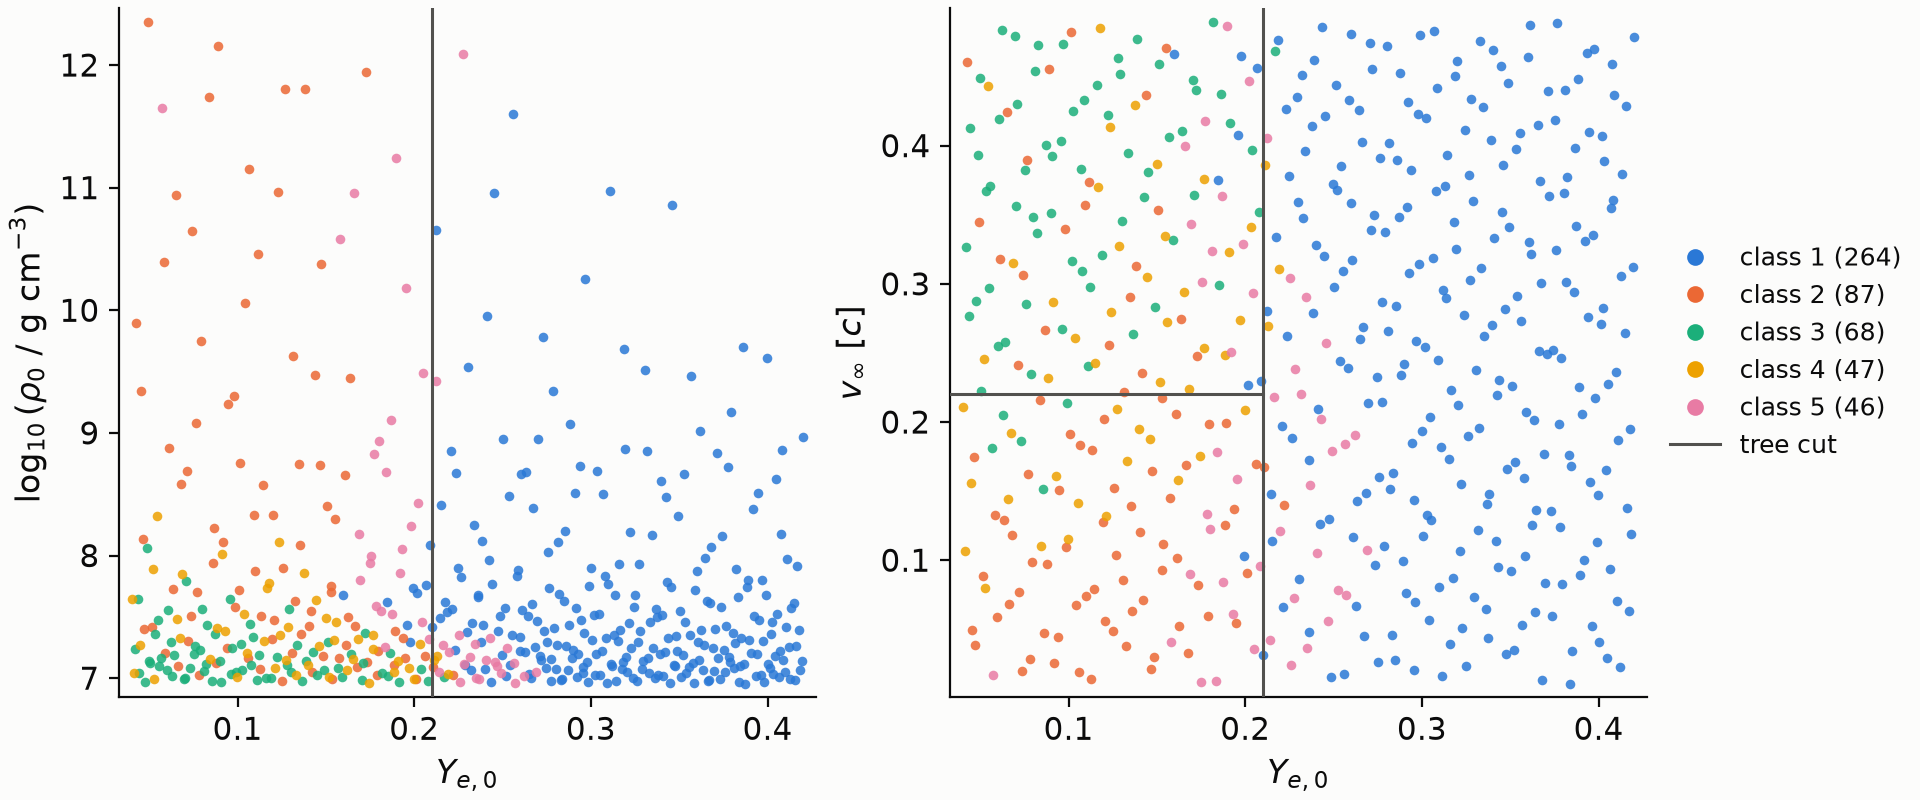
\includegraphics[width=\textwidth]{Figures/ratio_classes_map.png}
  \caption{Projections of the ensemble on the coordinate planes of the parameter space, coloured by class. The dashed lines mark $Y_{e,0}=0.21$ and $v_\infty=0.22\,c$.}
  \label{fig:res_class_map}
\end{figure}

The classes are organized mainly by the electron fraction and, below it, by the expansion.
Class~1 contains half of the box.
Of its 252 trajectories, 243 have $Y_{e,0}\geq0.21$, but it extends down to $Y_{e,0}=0.16$ for intermediate entropies and fast expansions, so $Y_{e,0}$ alone does not decide whether a trajectory is insensitive to the decay rates.
Classes~2, 4 and~3 contain the neutron-rich trajectories, $Y_{e,0}\lesssim0.22$, and they follow each other along the direction of increasing entropy and decreasing expansion timescale.
This is the direction in which the number of seeds decreases (Eq.~\ref{eq:seed_scaling}) and in which the time available for the flow of matter through the closed shells becomes shorter.
Class~5 straddles $Y_{e,0}\approx0.21$.
Even though we have five classes with two cuts, $Y_{e,0}=0.21$ and $v_\infty=0.22\,c$, we can reproduce the location of three large classes that contain the relevant physics conditions.
High electron fraction and low electron fraction with high velocity or low velocity.  
From those groups we can find the average and the ratios for each prescription.
Let us analyze the results class by class.

\paragraph{Class 1: $\beta^-$ heating at high electron fraction.}
In this subset of trajectories all three prescriptions produce a total effective heating rate dominated by $\beta^-$  decay.
The relevant nuclei from consistent across prescriptions are ${}^{132}$I and ${}^{127}$Sb both corresponds to the decay chains:

\begin{equation}\label{chain:I132}
  {}^{132}\mathrm{Te}\xrightarrow[3.2 \, {\rm d}] {\beta^{-}}{}^{132}\mathrm{I} \xrightarrow[2.28 \, {\rm h}] {\beta^{-}}{}^{132}\mathrm{Xe}\,\,\,\text{(stable)}
\end{equation}
\begin{equation}\label{chain:Sb127}
  {}^{127}\mathrm{Sb}\xrightarrow[3.8 \, {\rm d}] {\beta^{-}}{}^{127}\mathrm{Te} \xrightarrow[9.35 \, {\rm h}] {\beta^{-}}{}^{127}\mathrm{I}\,\,\,\text{(stable)}
\end{equation}
The leading heaters are the isobars of the second peak, $A=131$--$133$, together with $A=127$.
Since these isobars cannot be reached by $\alpha$ decay and fission is absent.
At the same time Fig.~\ref{fig:class_1_epsilon_ratios} shows that all the prescriptions have similar total effective heating rate and ratios between decay modes. 
\begin{figure}[H]
  \centering
  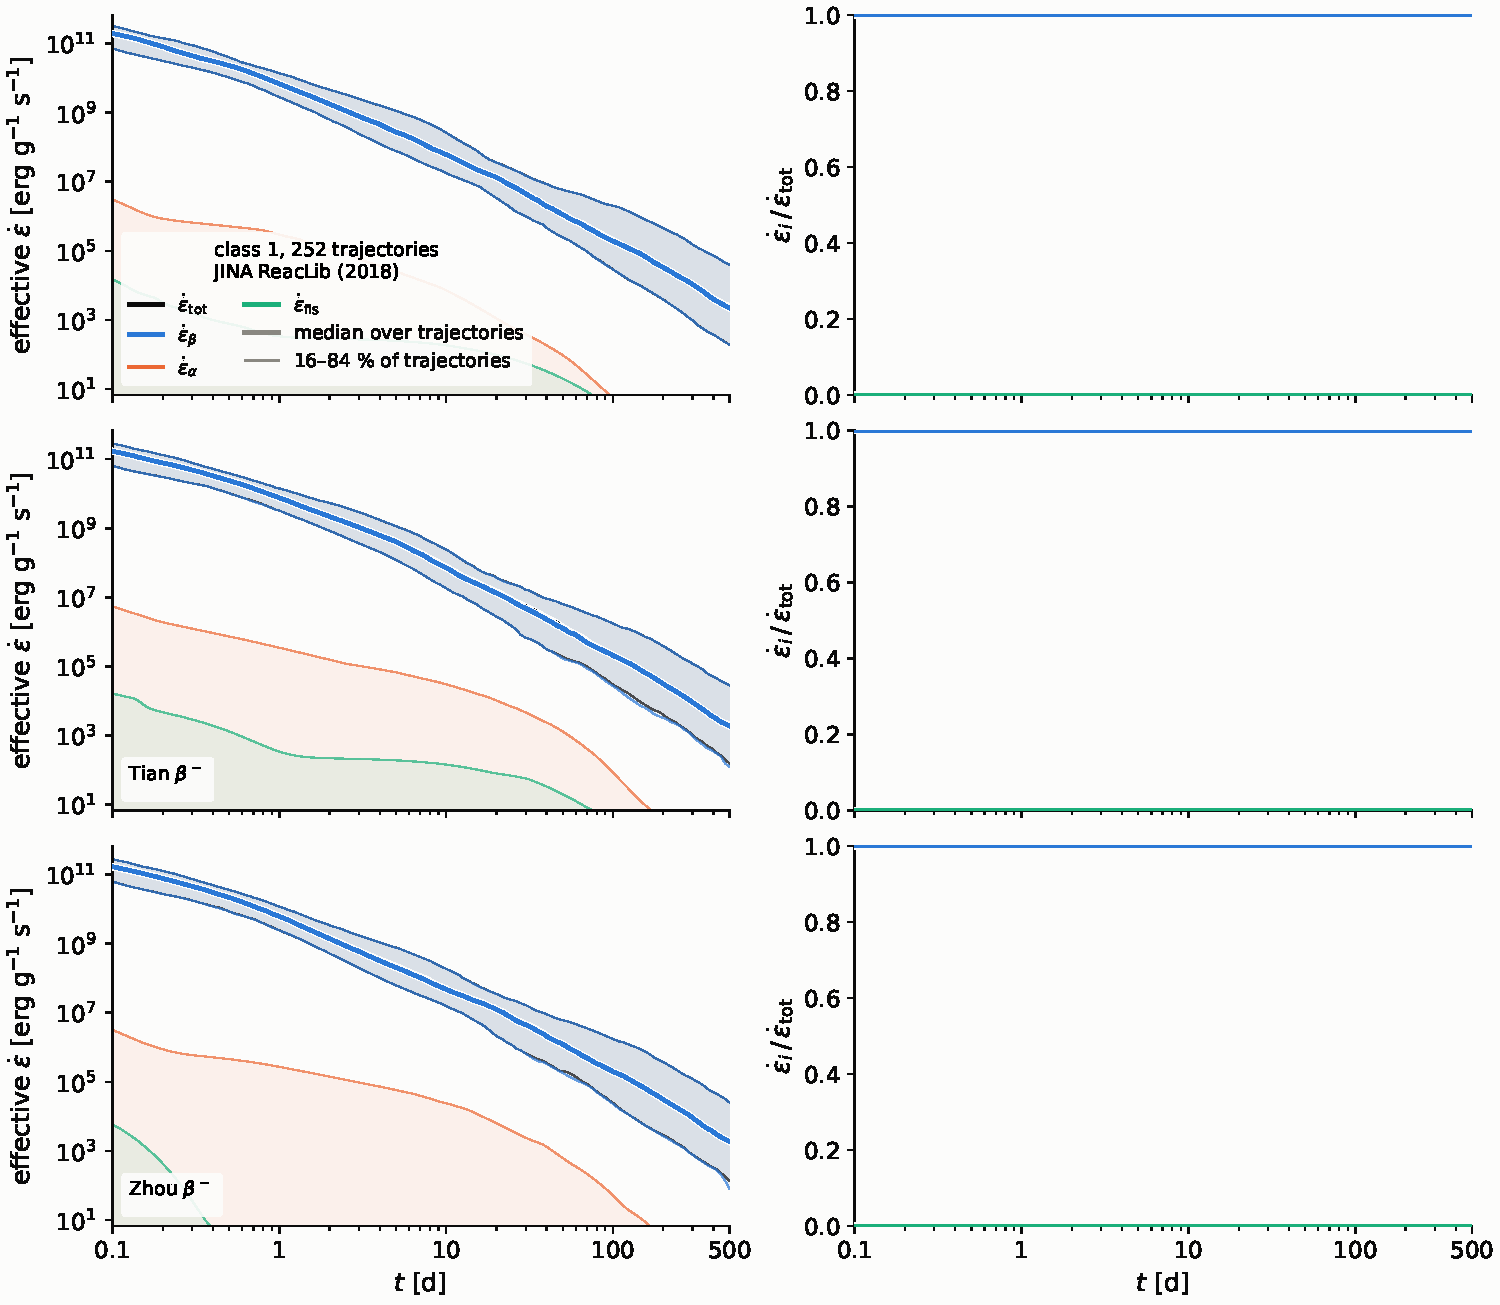
\includegraphics[width=0.8\textwidth]{Figures/heating_channels_sets_therm_class1.pdf}
  \caption{Average and spread of the total, $\alpha$,$\beta$ and fission effective heating rate per prescription across trajectories from class 1.}
  \label{fig:class_1_epsilon_ratios}
\end{figure}

\paragraph{Class 2: fission cycling in slow ejecta.}
Class~2 is the slowest class (median $v_\infty=0.14\,c$) and contains the most neutron-rich trajectories (median $Y_{e,0}=0.12$), the regime of fission cycling (Sec.~\ref{sec:fission}).
It shows the largest deviations of the total effective heating rate between prescriptions (see Fig.~\ref{fig:class_2_epsilon_ratios_prep}).
The ratio between Tian and Zhou is of the order of $20$ with trajectories reaching up to $40$.
This is not because Tian produce more heating but because Zhou does not.
Fission carries a third of the Tian energy and a quarter of the ReacLib energy, but only $0.3\%$ of the Zhou energy.
The $\alpha$ channel releases a comparable energy in the three sets, but with a different composition.
In ReacLib and Tian it contains the $A\geq240$ emitter ${}^{253}$Es (and, in ReacLib, ${}^{252}$Cf) with decay chains:

\begin{equation}
  ^{253}\mathrm{Es} \xrightarrow[20.5 \, {\rm d}] {\alpha}{}^{249}\mathrm{Bk} \xrightarrow[327.2 {\rm \, d}] {\beta} ^{249}\mathrm{Cf} \xrightarrow [351 \,{\rm y}] {\alpha} \cdots 
\end{equation}
\begin{equation}
  {}^{252}\mathrm{Cf} \xrightarrow[2.65 \, {\rm y}] {\alpha}{}^{248}\mathrm{Cm} \xrightarrow[3.48 \times 10^{5} {\rm \, y}] {\alpha} \cdots 
\end{equation}

In Zhou these are absent and the odd-$A$ series headed by ${}^{225}$Ac and ${}^{223}$Ra dominate.
\begin{equation}
  {}^{225}\mathrm{Ac} \xrightarrow[9.91\,\mathrm{d}]{\alpha}{}^{221}\mathrm{Fr} \xrightarrow[4.8\,\mathrm{min}]{\alpha}{}^{217}\mathrm{At}
\end{equation}
\begin{equation}
  {}^{223}\mathrm{Ra} \xrightarrow[11.44 \, {\rm d}] {\alpha}{}^{219}\mathrm{Rn} \xrightarrow[3.96 {\rm \, s}] {\alpha} {}^{215}\mathrm{Po}
\end{equation}
The $A\geq240$ material releases its energy mainly by spontaneous fission, 10--18 times more than through the $\alpha$ decays of ${}^{253}$Es and ${}^{252}$Cf.
Since Tian and Zhou share the $\alpha$ rates, the absence of late-time fission in Zhou is an effect of the $\beta^-$ rates.

\begin{figure}[H]
  \centering
  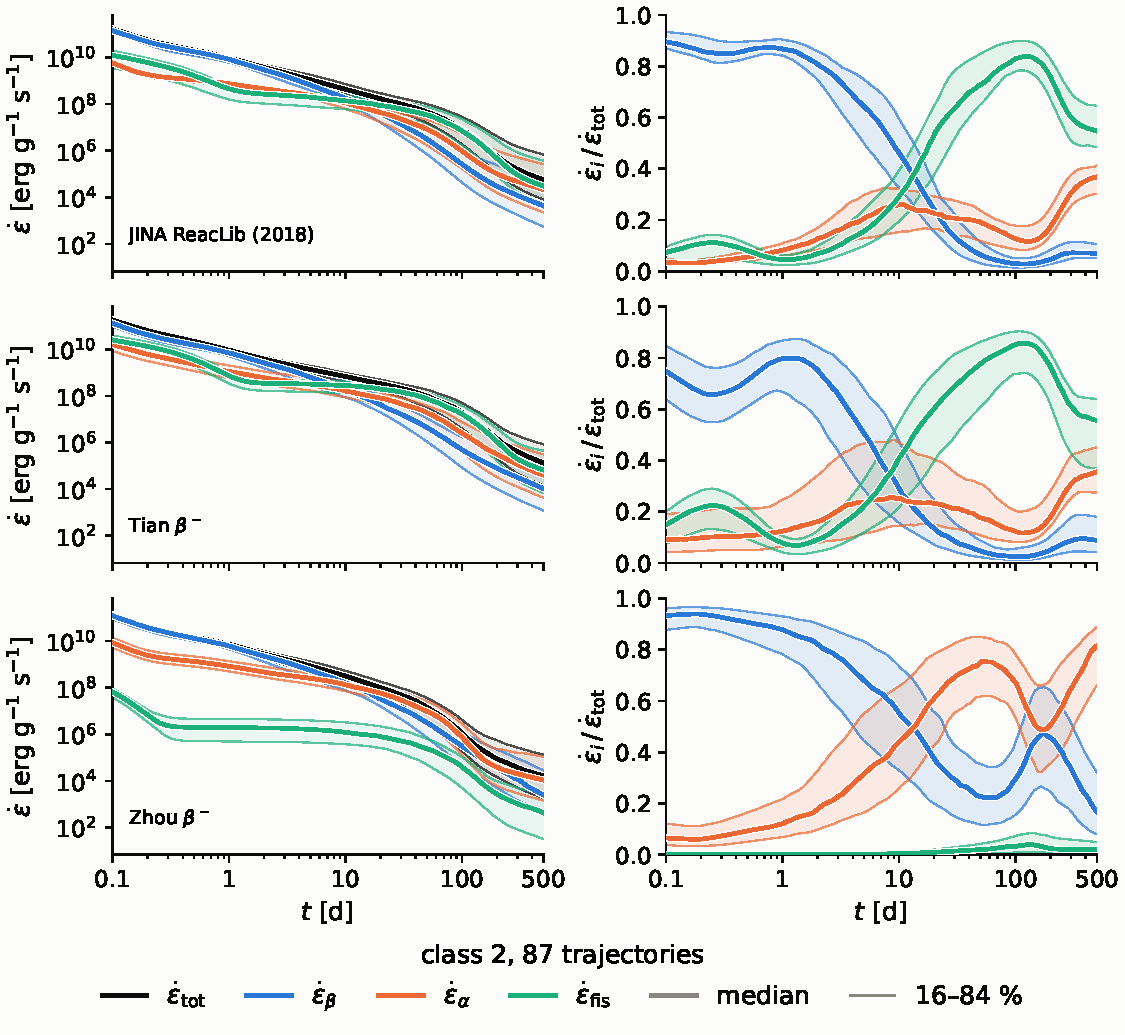
\includegraphics[width=0.8\textwidth]{Figures/heating_channels_sets_therm_class2.pdf}
  \caption{Average and spread of the total, $\alpha$,$\beta$ and fission effective heating rate per prescription across trajectories from class 2.}
  \label{fig:class_2_epsilon_ratios}
\end{figure}
\begin{figure}[H]
  \centering
  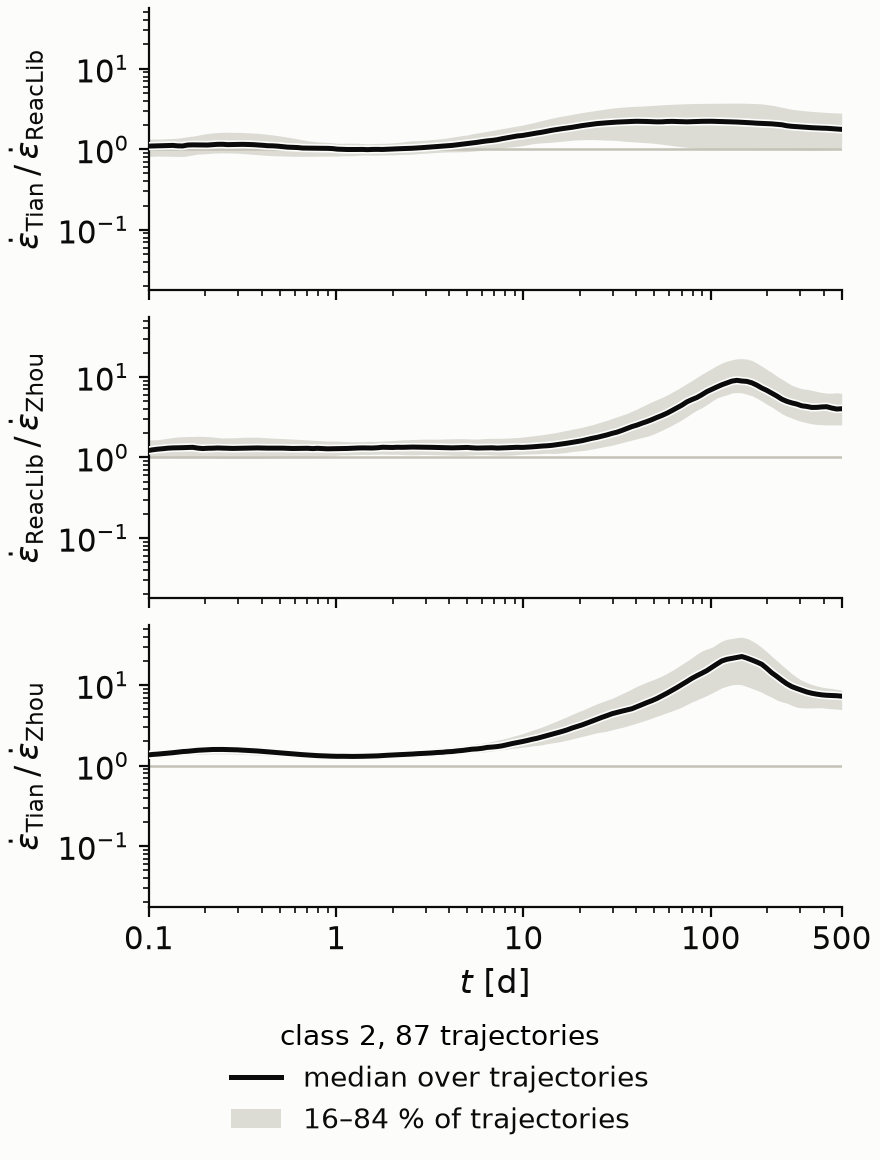
\includegraphics[width=0.5\textwidth]{Figures/heating_ratios_sets_therm_class2.png}
  \caption{Average and spread of the  ratio of the effective heating rate between prescriptions across trajectories from class 2.}
  \label{fig:class_2_epsilon_ratios_prep}
\end{figure}

\paragraph{Class 3: fast, high-entropy, neutron-rich ejecta.}
Class~3 collects the fastest (median $v_\infty=0.38\,c$) and highest-entropy ($s_0\geq13$, median 37) neutron-rich trajectories, which also have the lowest initial densities.
Under these conditions part of the neutrons are not captured (Sec.~\ref{sec:methods_start}).
This cause a rapid increase of $Ye$ at the timescale of the halflife of free neutrons (see Fig.~\ref{fig:trajectories_T_Ye}).
No set produces late-time fission (see Fig.~\ref{fig:class_3_epsilon_ratios}).

The empirical sets release more energy than ReacLib (see Fig.~\ref{fig:class_3_epsilon_ratios_prep}).
Tian and Zhou agree in the $\alpha$ channel while Reaclib do not have the $\alpha$ peak in the ratio between 10 and 100 d.
The relevant decay chains appears on all prescriptions for $\alpha$ are:
\begin{equation}
  {}^{224}\mathrm{Ra} \xrightarrow[3.63 \, {\rm d}] {\alpha}{}^{220}\mathrm{Rn} \xrightarrow[55.6 {\rm \, s}] {\alpha} {}^{216}\mathrm{Po}\xrightarrow[144 {\rm \, ms}] {\alpha} {}^{212}\mathrm{Pb}\xrightarrow[10.6 {\rm \, h}] {\beta^{-}} {}^{212}\mathrm{Bi}.
\end{equation}
${}^{212}$Bi Have two decay paths, it can go to ${}^{212}$Po through $\beta^{-}$ decay or ${}^{208}$Tl through $\alpha$ decay.
Both path ends on ${}^{208}$Pb.
The mayor difference between prescriptions is that 
Zhou and Tain have contributions from the odd $A$ chain:
\begin{equation}
    {}^{223}\mathrm{Ra} \xrightarrow[11.44 \, {\rm d}] {\alpha}{}^{219}\mathrm{Rn} \xrightarrow[3.96 {\rm \, s}] {\alpha} {}^{215}\mathrm{Po}\xrightarrow[1.7 {\rm \, ms}] {\alpha} {}^{211}\mathrm{Pb}\xrightarrow[36.1 {\rm \, min}] {\beta^{-}} {}^{211}\mathrm{Bi}\xrightarrow[2.1 {\rm \, min}] {\alpha} {}^{207}\mathrm{Tl}\xrightarrow[4.77 {\rm \, min}] {\beta^{-}} {}^{207}\mathrm{Pb}\,\,\text{(stable)}.
\end{equation}
\begin{figure}[H]
  \centering
  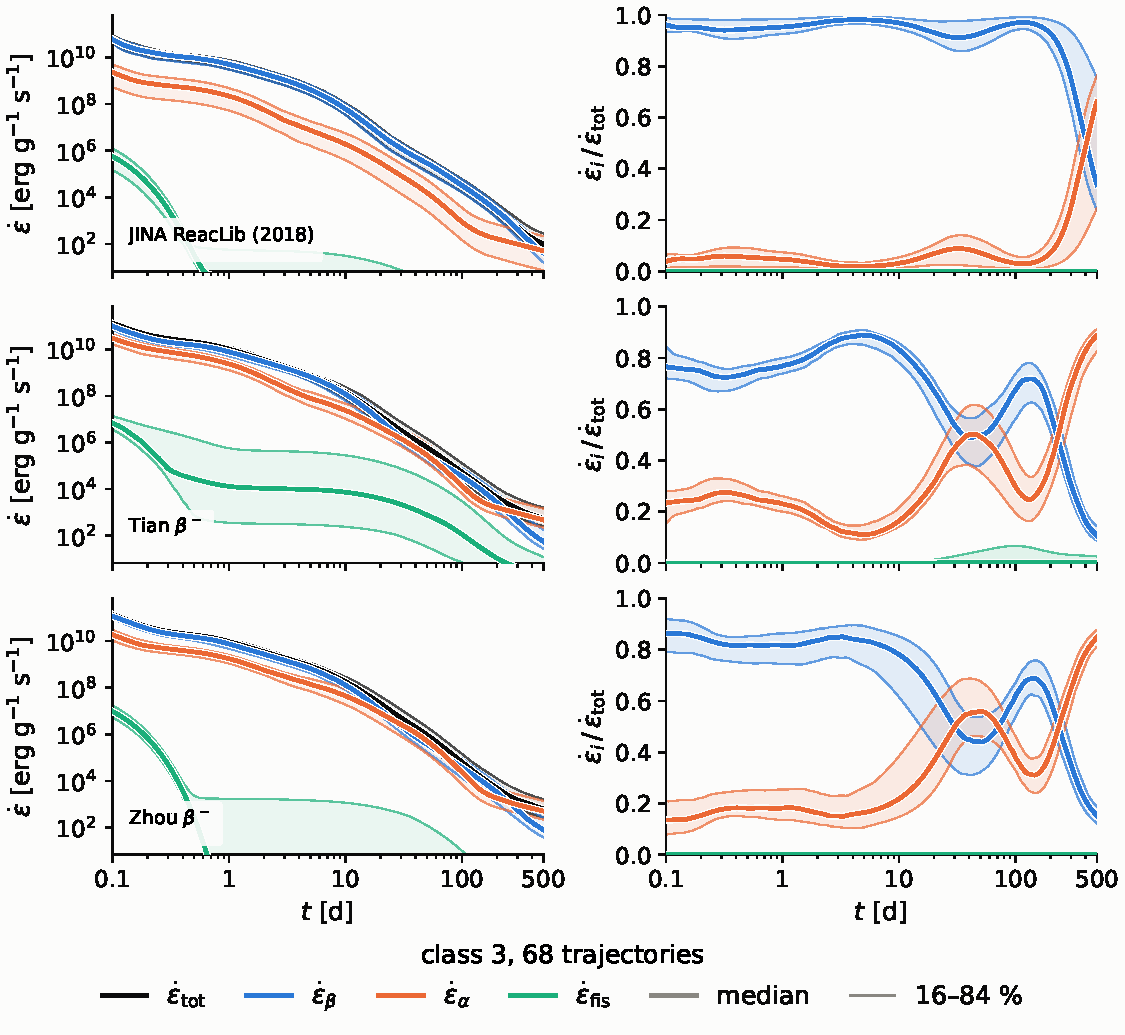
\includegraphics[width=0.8\textwidth]{Figures/heating_channels_sets_therm_class3.pdf}
  \caption{Average and spread of the total, $\alpha$,$\beta$ and fission effective heating rate per prescription across trajectories from class 3.}
  \label{fig:class_3_epsilon_ratios}
\end{figure}
\begin{figure}[H]
  \centering
  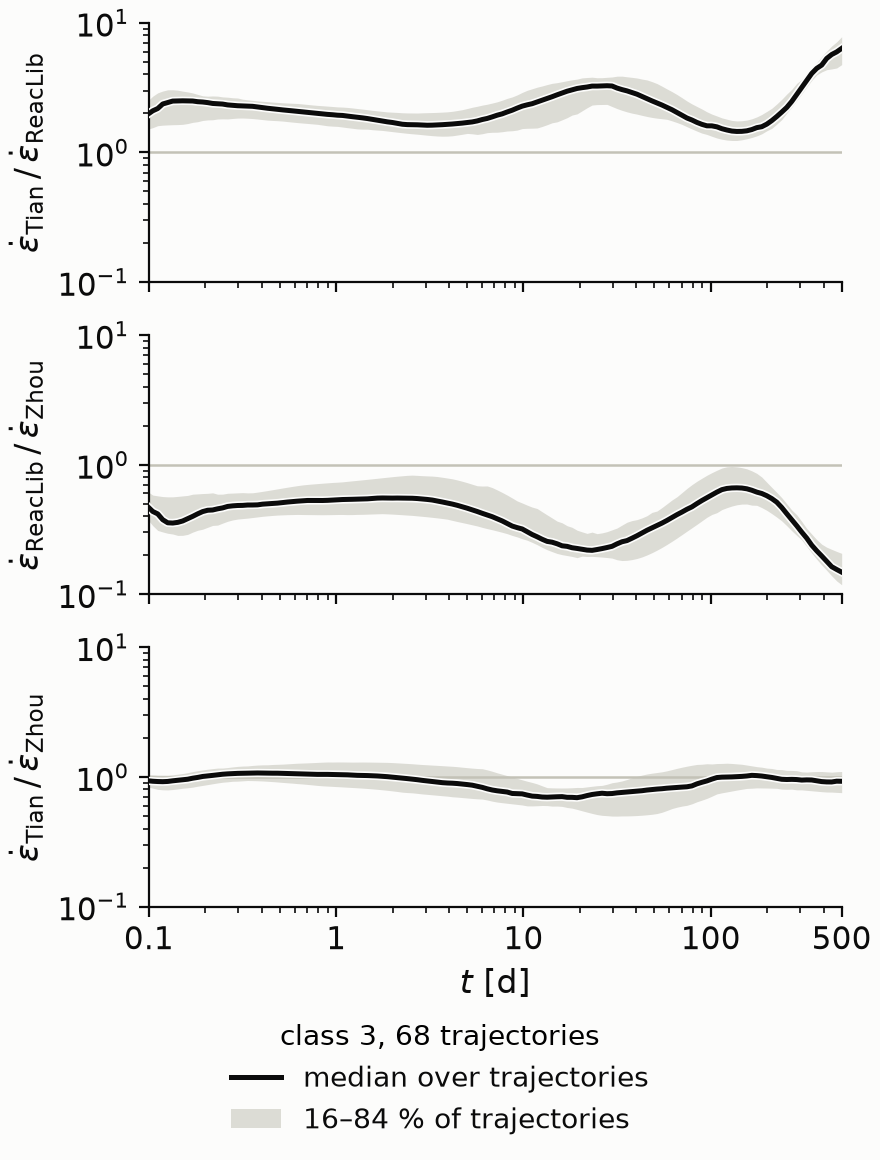
\includegraphics[width=0.6\textwidth]{Figures/heating_ratios_sets_therm_class3.png}
  \caption{Average and spread of the  ratio of the effective heating rate between prescriptions across trajectories from class 3.}
  \label{fig:class_3_epsilon_ratios_prep}
\end{figure}
%--------------------------------------------------------------------
\paragraph{Class 4: three prescriptions, three channels.}
Class~4 lies between classes~2 and~3 (median $s_0=29$, $v_\infty=0.25\,c$), and here each set heats through a different combination of channels.
ReacLib heats almost only by $\beta^-$ decay, half of it in the isobar $A=202$ (${}^{202}$Pt$\to{}^{202}$Au) on the high-mass side of the third peak.
Tian adds fission and $\alpha$ decay while Zhou only adds $\alpha$ decay alone carried by the odd-$A$ series.
Form Fig.~\ref{fig:class_4_epsilon_ratios_prep} we find that Tian has higher total effective heating rate compared with Reaclib mainly because the fission contribution.
On the other hand, Zhou has higher contribution from $\alpha$ decay.
That means that in this class each prescription has its own preference for the decay mode.
\begin{figure}[H]
  \centering
  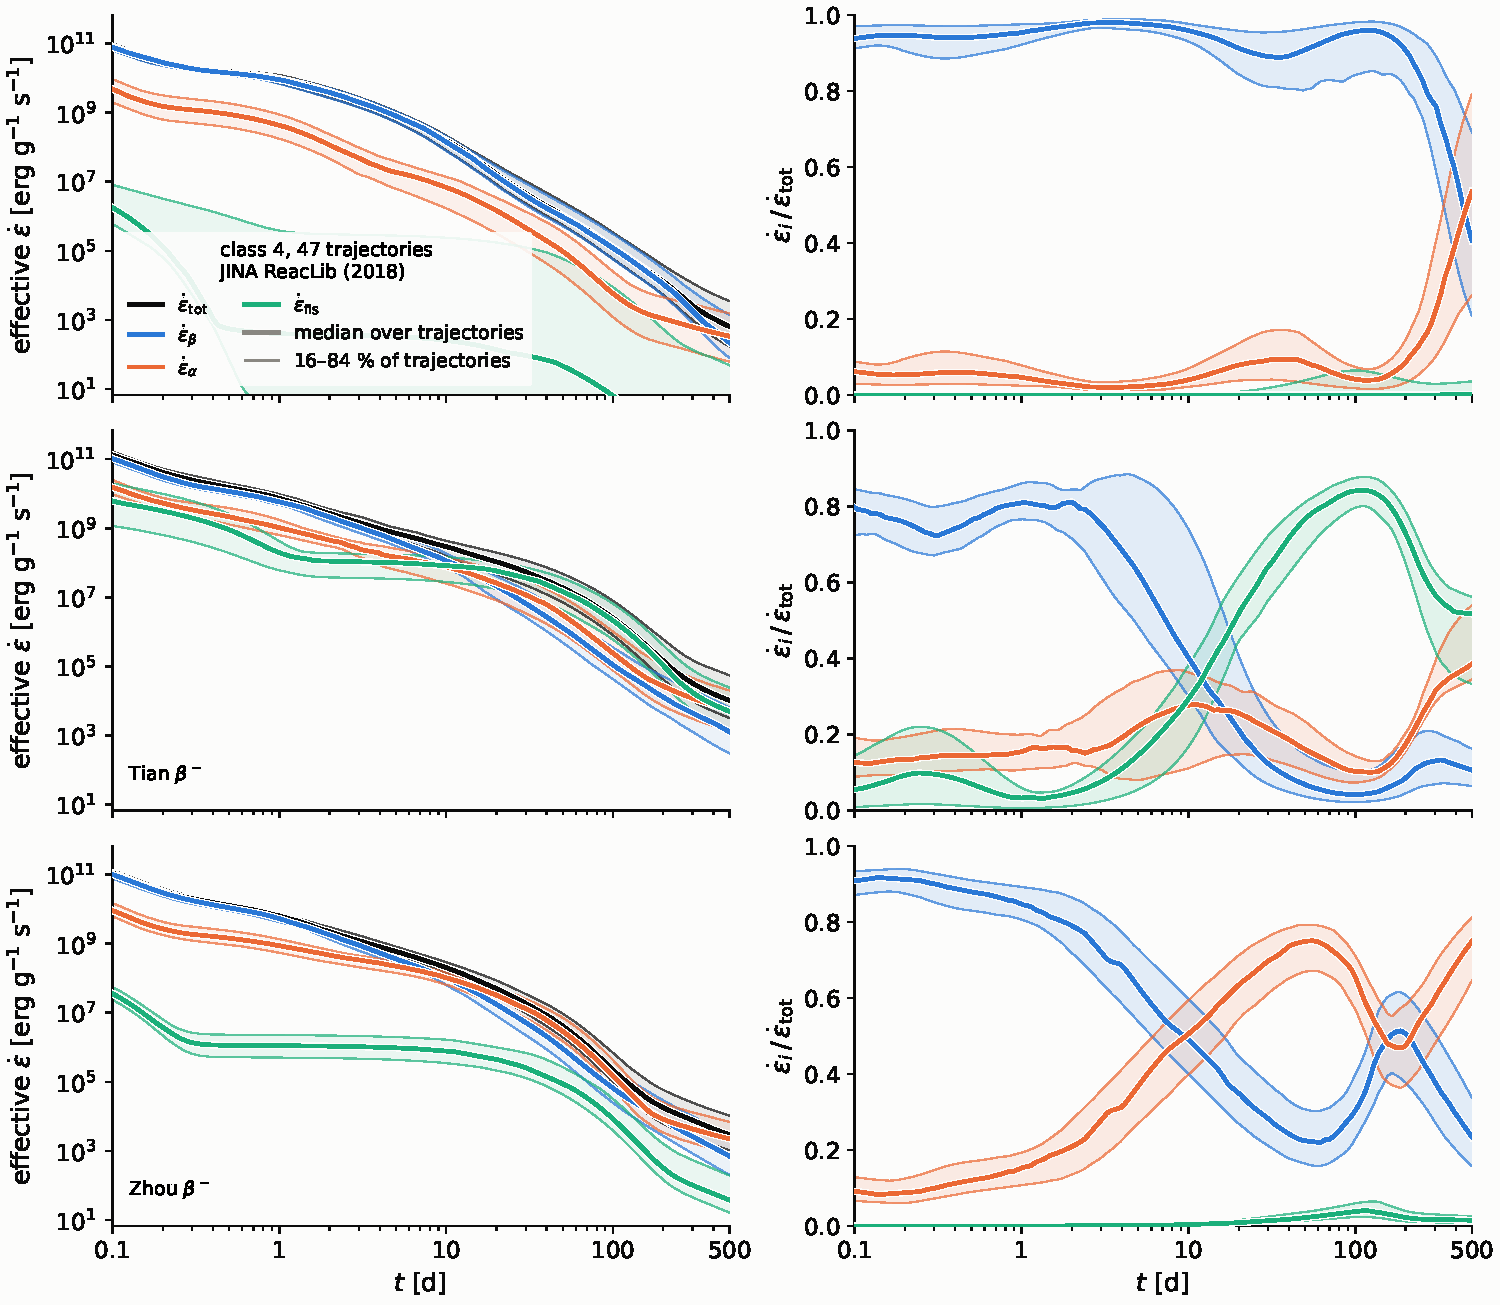
\includegraphics[width=0.8\textwidth]{Figures/heating_channels_sets_therm_class4.pdf}
  \caption{Average and spread of the total, $\alpha$,$\beta$ and fission effective heating rate per prescription across trajectories from class 4.}
  \label{fig:class_4_epsilon_ratios}
\end{figure}
\begin{figure}[H]
  \centering
  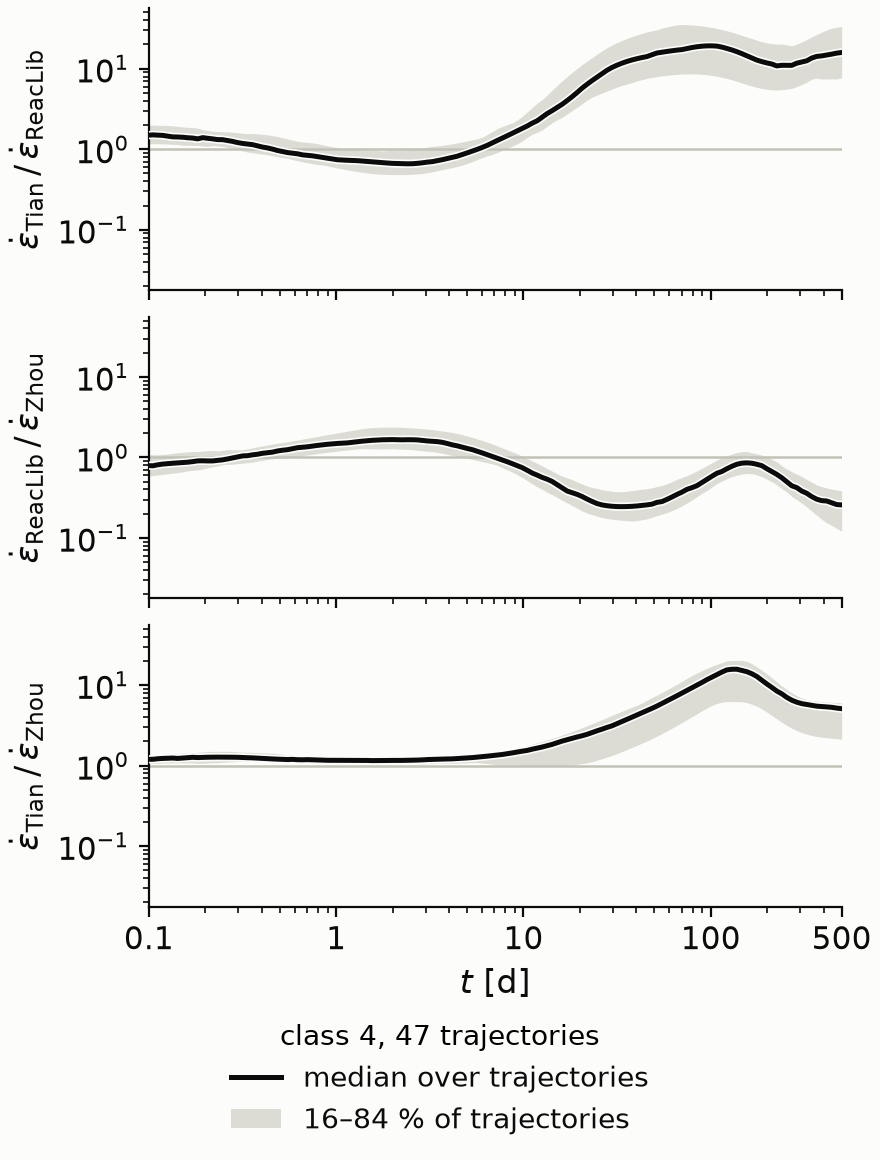
\includegraphics[width=0.6\textwidth]{Figures/heating_ratios_sets_therm_class4.png}
  \caption{Average and spread of the  ratio of the effective heating rate between prescriptions across trajectories from class 4.}
  \label{fig:class_4_epsilon_ratios_prep}
\end{figure}

\paragraph{Class 5: the boundary.}
Class~5 lies on $Y_{e,0}\approx0.21$ and spans the full range of entropies and velocities.
We can understand this class as a transition between the class~1 with only $\beta^{-}$ decays to classes 2, 3 and 4.
The main difference between prescriptions are found between Zhou and Reaclib where Reaclib has fission contribution while zhou does not.
\begin{figure}[H]
  \centering
  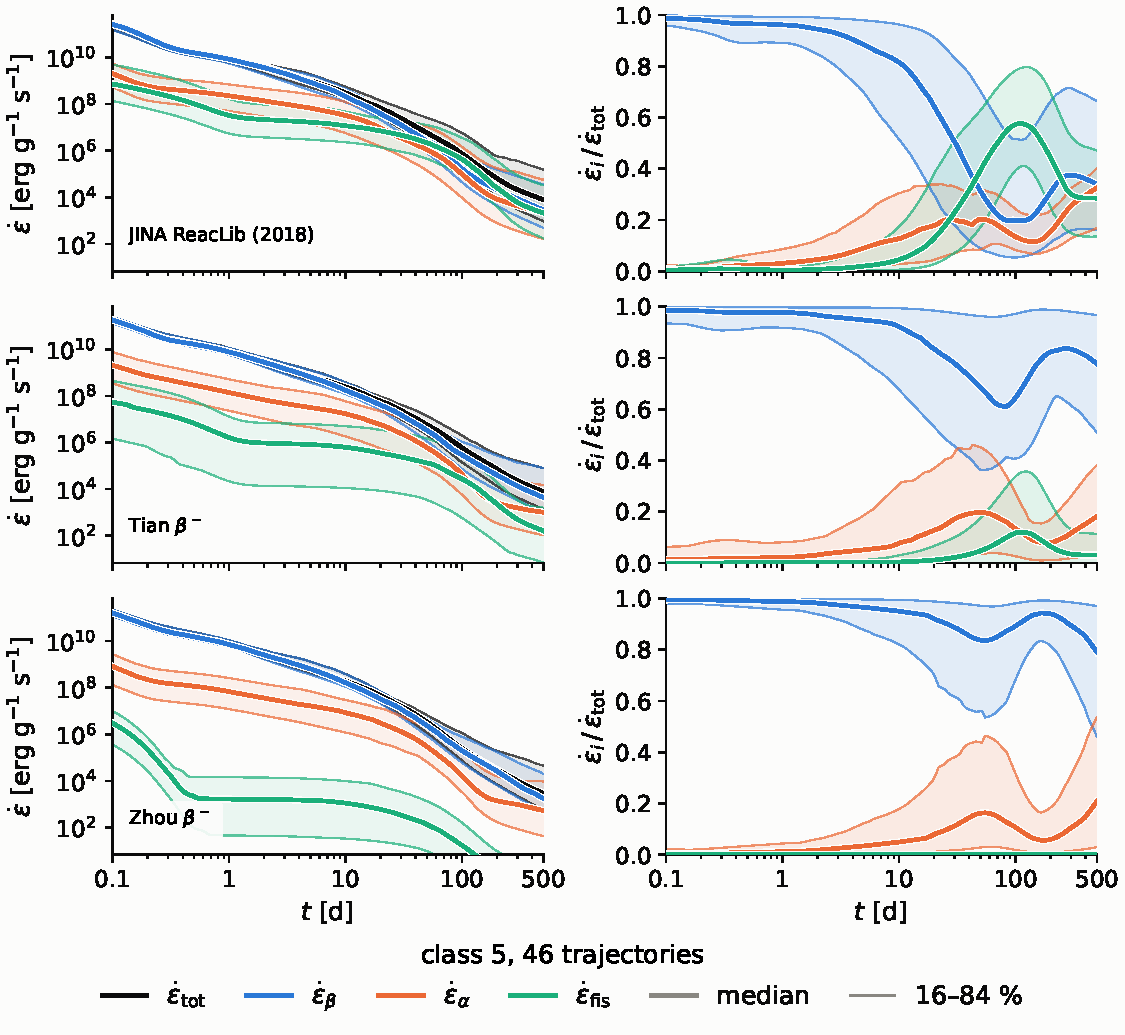
\includegraphics[width=0.8\textwidth]{Figures/heating_channels_sets_therm_class5.pdf}
  \caption{Average and spread of the total, $\alpha$,$\beta$ and fission effective heating rate per prescription across trajectories from class 5.}
  \label{fig:class_5_epsilon_ratios}
\end{figure}
\begin{figure}[H]
  \centering
  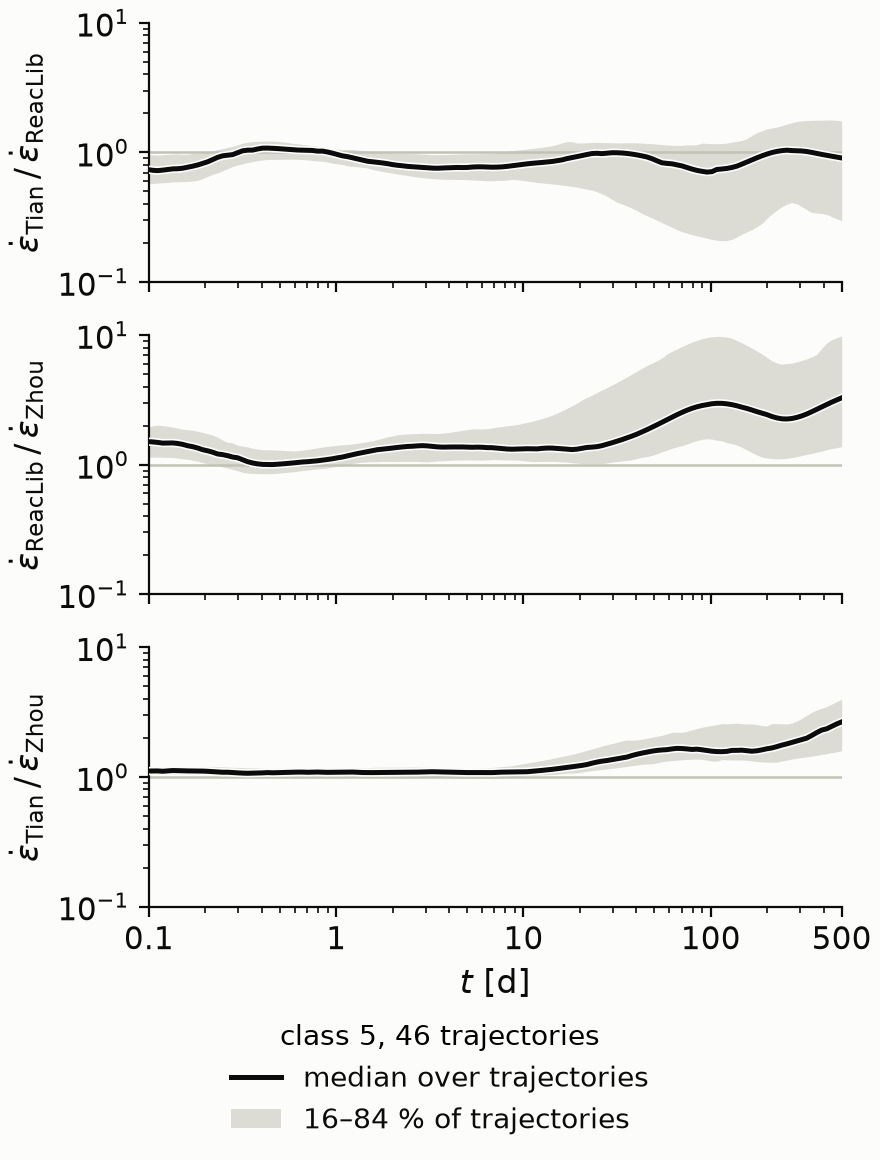
\includegraphics[width=0.6\textwidth]{Figures/heating_ratios_sets_therm_class5.png}
  \caption{Average and spread of the  ratio of the effective heating rate between prescriptions across trajectories from class 5.}
  \label{fig:class_5_epsilon_ratios_prep}
\end{figure}
----------------------

%------------------------------------------------------------------------------------------
\section{Origin of the dependence on the decay rates}\label{sec:res_origin}
%------------------------------------------------------------------------------------------

Since the relevant nuclei themselves have measured decays, the differences between the sets are differences in where the matter ends.
The prescription moves matter between three mass regions: the second peak ($A\approx125$--$133$), the high-mass side of the third peak ($A\approx202$) and the region of the $\alpha$ emitters and actinides ($A\gtrsim220$).
Figure~\ref{fig:res_abund} shows the corresponding abundance patterns.

%%%%%%%%%%%%%%%%%  figure: abundances  %%%%%%%%%%%%%%%%%

\begin{figure}[H]
\centering
\subfloat[]{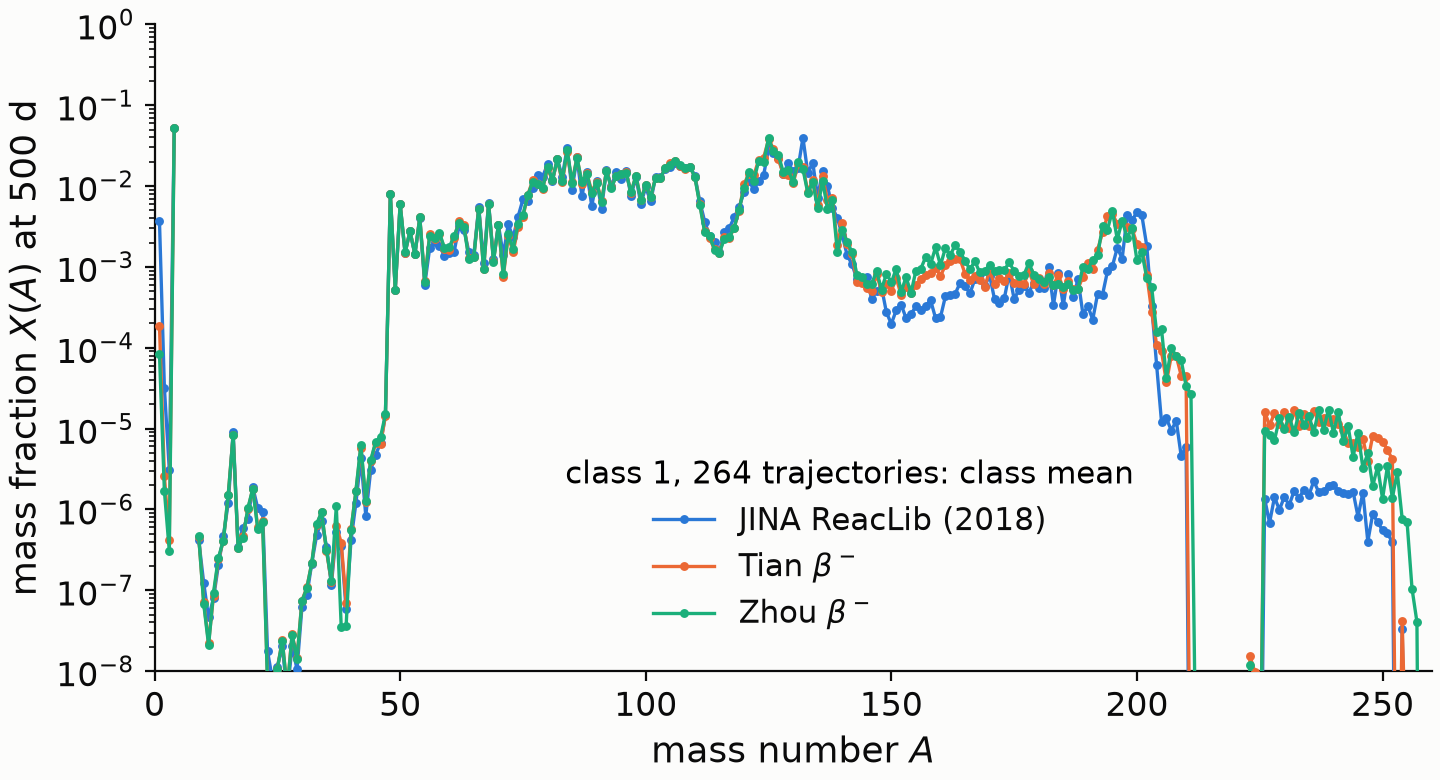
\includegraphics[width=0.5\textwidth]{Figures/abundances_class1.png}}\hfil
\subfloat[]{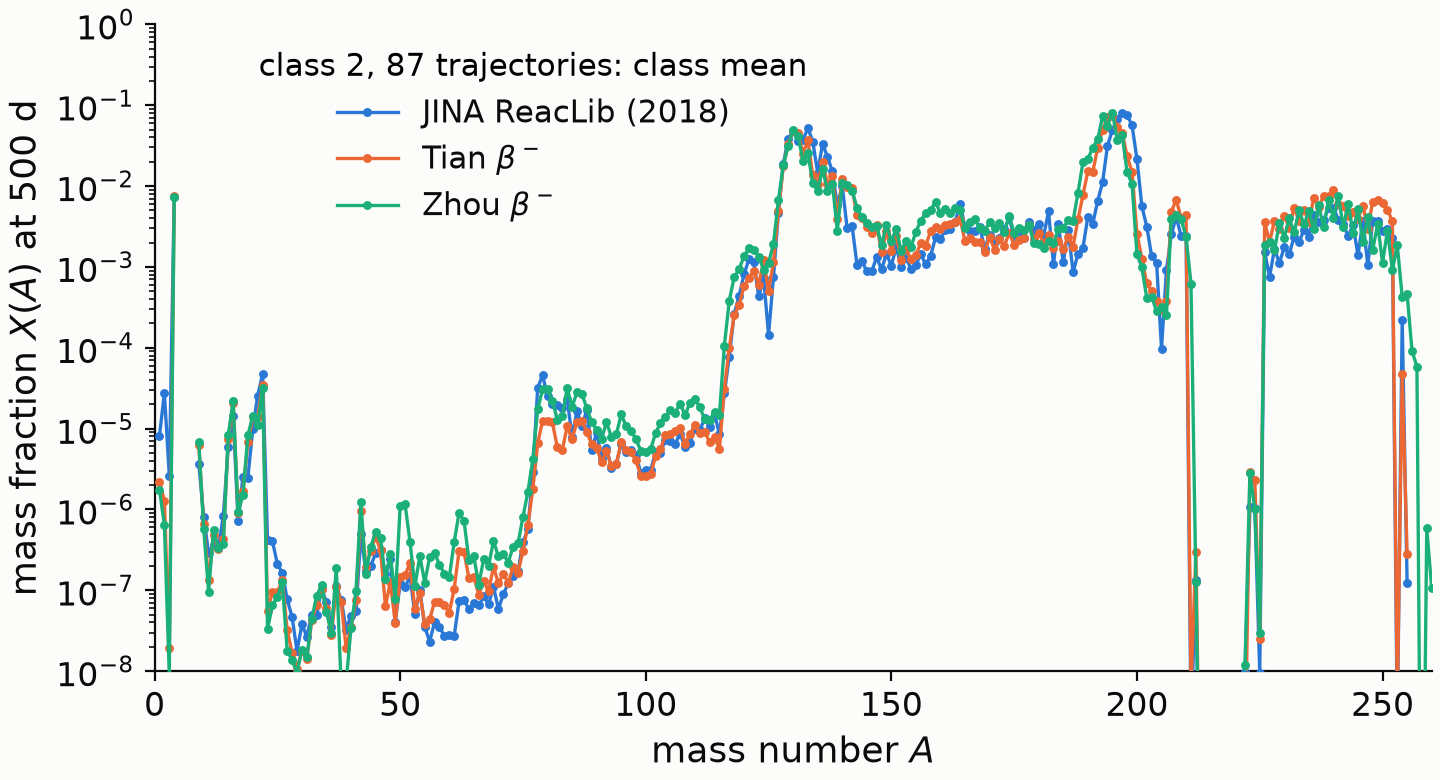
\includegraphics[width=0.5\textwidth]{Figures/abundances_class2.png}}

\subfloat[]{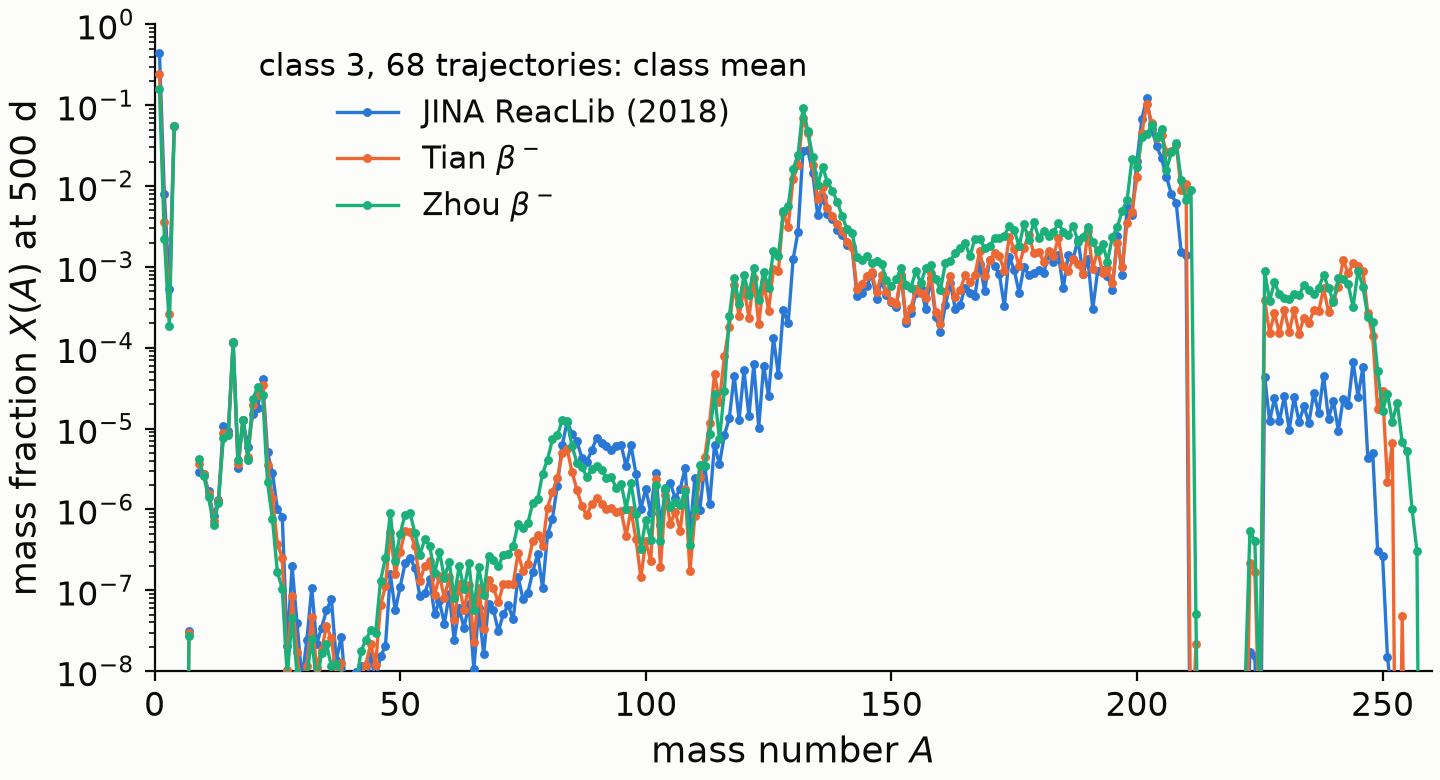
\includegraphics[width=0.5\textwidth]{Figures/abundances_class3.png}}\hfil
\subfloat[]{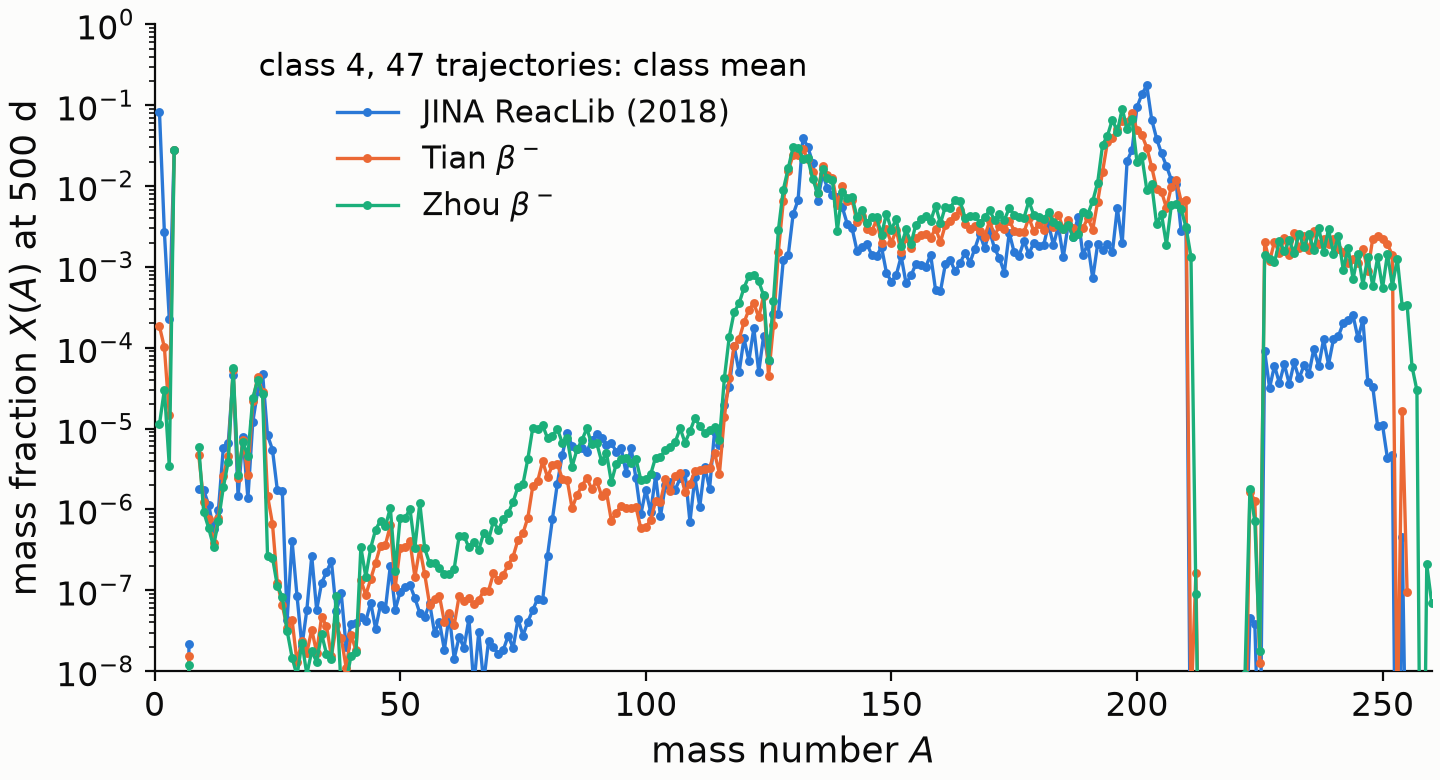
\includegraphics[width=0.5\textwidth]{Figures/abundances_class4.png}}%

\subfloat[]{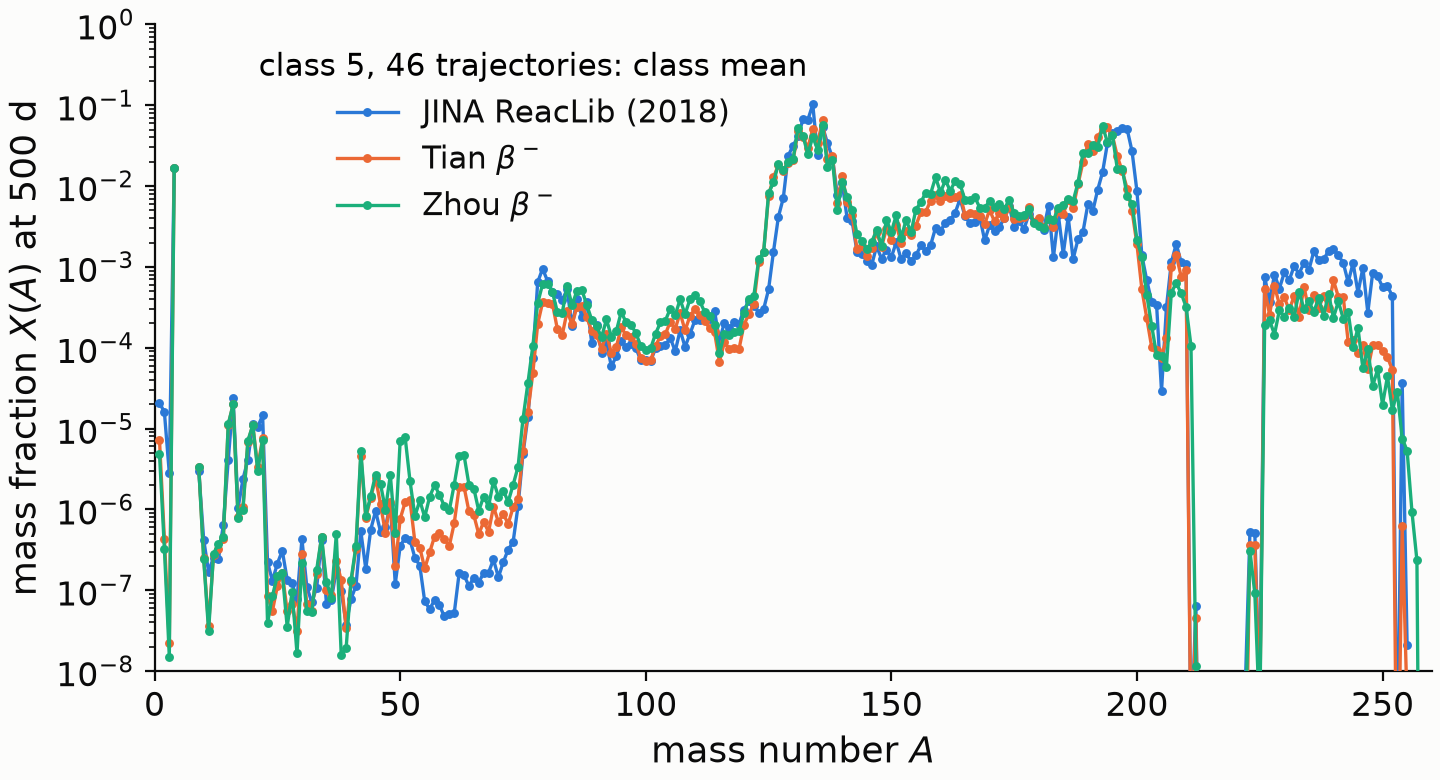
\includegraphics[width=0.5\textwidth]{Figures/abundances_class5.png}}
\caption{Abundances for the different classes of thermodynamic trajectories.}\label{Abundances}

\end{figure}

The second-peak isobars are richer in ReacLib than in the empirical sets in every class except class~3: by factors of $2.3$--$2.4$ in class~1, $1.3$--$1.6$ in class~2, $1.3$--$1.5$ in class~4 and $1.6$ in class~5, and by about two at $A=125$--$128$ in class~6 (before the correction of the neutrino losses).
In classes~3 and~4 ReacLib retains much more matter at $A=202$, while the empirical sets carry more matter to $A\gtrsim220$; in class~3 they also produce more matter at the second peak.
The $\beta^-$ rates of the closed-shell nuclei set how much matter accumulates in the peaks and how fast it moves past them~\cite{mumpower_impact_2016}, and most of these numbers are consistent with one reading: compared with the two empirical formulae, FRDM+QRPA retains matter longer at the closed shells $N=82$ and $N=126$.
At high $Y_e$ this leaves more matter at $A\approx127$--$133$ (classes~1, 5 and~6).
In fast neutron-rich trajectories, where the time available for the flow is short ($\tau\approx0.4$--$0.6\,\mathrm{ms}$), it keeps matter at $A\approx202$, so that less matter reaches $A\gtrsim220$ (classes~3 and~4).
In class~3 the matter that passes $N=126$ in the empirical sets reaches the fissioning nuclei, whose fragments would explain their richer second peak.
This reading does not explain why ReacLib produces the most actinides in class~5.
It also rests on unmeasured half-lives.
It must be checked against the ratios of the empirical and FRDM+QRPA half-lives along $N=82$ and $N=126$ (Fig.~\ref{fig:rate_comparison})  and against Fig.~\ref{fig:res_abund}.

In the slower trajectories of class~2, all three sets carry matter past $N=126$, and the difference moves to the survival of the $A\geq240$ material.
There the clean comparison is between Tian and Zhou.
With identical $\alpha$ rates, Tian retains enough $A\geq240$ material to make fission a third of its released energy, whereas Zhou retains essentially none.
In no class does Zhou release more than $0.3\%$ of its energy by fission.
The budgets do not decide whether this happens because the flow in Zhou stops below $A\approx240$, or because the $A\geq240$ material is destroyed during the decay to stability.
The time evolution of $X_{A\geq240}$ and the abundances for $A=220$--$260$ at $1\,\mathrm{s}$ and $1\,\mathrm{d}$ distinguish the two .
The enhanced odd-$A$ $\alpha$ series of Zhou in classes~2 and~4, which requires matter at $A\approx223$--$229$, is consistent with the first.

\section{Luminosity}
\begin{figure}[H]
  \centering
  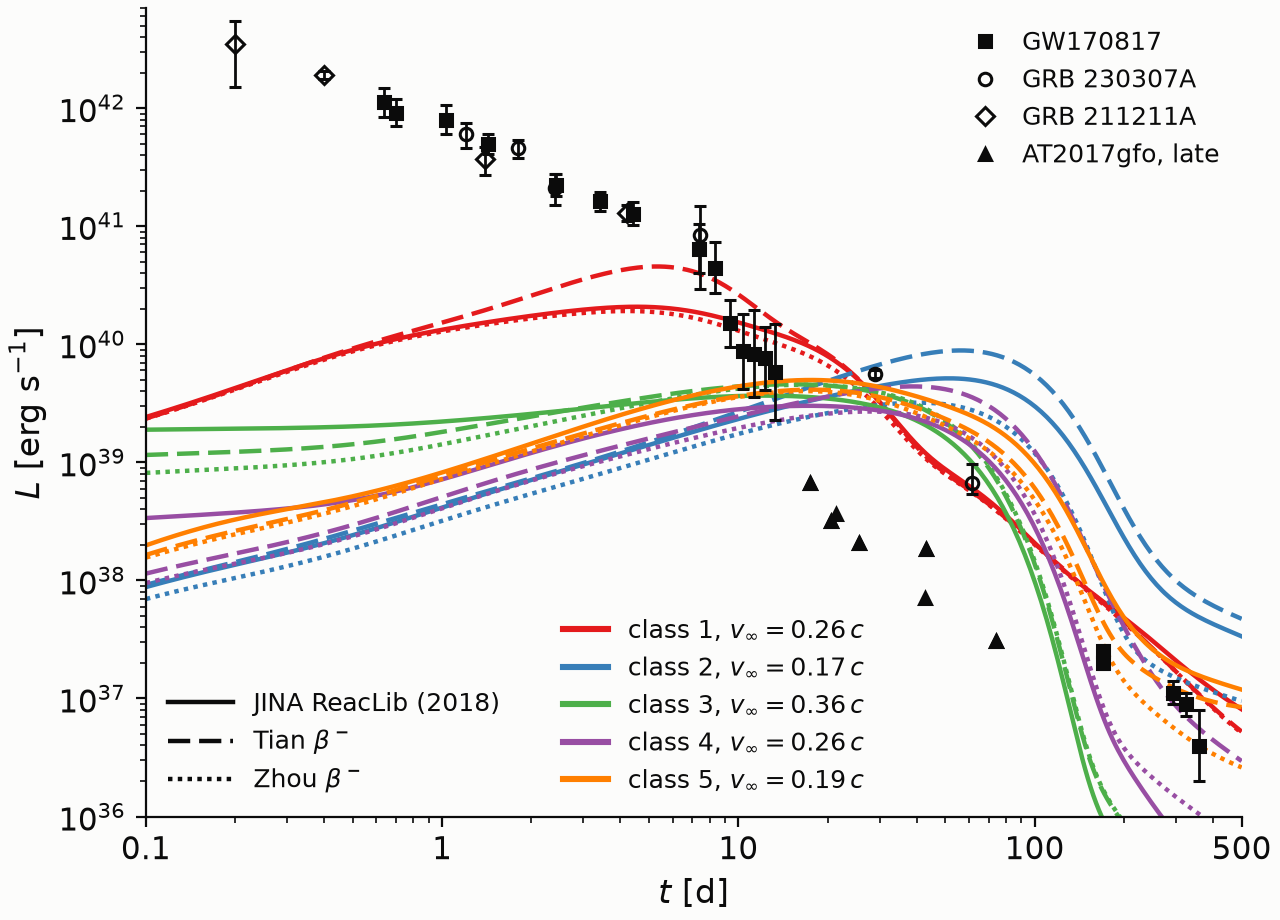
\includegraphics[width=0.6\textwidth]{Figures/luminosity_classes_Ye_v.png}
  \caption{Bolometric luminosity as a function of time for each prescription and class.}
  \label{fig:Luminosity}
\end{figure}
-------------


%------------------------------------------------------------------------------------------
\section{Summary}\label{sec:res_nucleo_summary}
%------------------------------------------------------------------------------------------

\begin{enumerate}
  \item The response of the heating to the decay rates falls into six regimes.
  The three large ones are located by two cuts, $Y_{e,0}=0.21$ and $v_\infty=0.22\,c$, and the other three are transitions or corners of the parameter space.
  \item Half of the box (class~1) is the least sensitive, but not insensitive.
  Once the spurious decays of ${}^{48}$Ca and ${}^{96}$Zr are removed from the Tian set, the two empirical formulae agree within about $5\%$ and lie about $20\%$ below FRDM+QRPA, through the second-peak isobars.
  \item The largest sensitivity occurs for $Y_{e,0}\lesssim0.21$.
  There the released energy differs by a factor of two (class~2, Tian/Zhou) or 1.7 (class~3, Zhou/ReacLib), and in class~4 each prescription heats through a different combination of channels.
  \item All leading heaters have measured decays, so the sensitivity is indirect: it acts through the abundances.
  \item The Zhou formula never retains $A\geq240$ material: late-time fission carries at most $0.3\%$ of its energy, against up to $34\%$ for Tian and $23\%$ for ReacLib.
  Since Tian and Zhou share the $\alpha$ rates, this is an effect of the $\beta^-$ rates.
  \item Where the $A\geq240$ material survives, it releases 10--18 times more energy by fission than by $\alpha$ decay.
  In Ref.~\cite{hernandez_porras_features_2027}, which excluded fission, the same material appeared through the $\alpha$ emitters ${}^{252}$Cf, ${}^{253}$Es, ${}^{254}$Es and ${}^{254}$Fm.
  \item The $\alpha$ heating is carried by the four decay series.
  The weight of the odd-$A$ series increases from ReacLib to Tian to Zhou in every class with an appreciable $\alpha$ channel.
\end{enumerate}